Snowball is a leaderless, multi-decree, probabilistic consensus protocol that makes
use of sub-sampled voting. It entangles voting results to render the process
more efficient than independently deciding on each item alone. We first provide
the intuition behind the protocol informally, then present the formal protocol
specification, followed by a proof of safety and discussion on liveness for virtuous
transactions.

\subsection{Intuition}

The protocol operates by building a directed acyclic graph (DAG) of all known transactions.
This DAG is rooted at a protocol-defined \emph{genesis} transaction shared by all nodes.
Each transaction is represented as a vertex in the DAG.
When a transaction is created, it names one or more \emph{parent transactions}, which point to already accepted vertices in the DAG.
The parent-child relationships encoded in the DAG do not correspond to application-specific structure; for instance, a child vertex need not spend or have any relationship with the funds received in the parent transaction.
These relationships exist solely to entangle and enforce the fate of previous decisions made by the system.
For each vertex in the resulting DAG, there exists a static \emph{ancestor set} that contains all transactions reachable via parent edges back in history, and a \emph{progeny} that recursively includes all children transactions and their offspring.

The central challenge in Snowball is to choose among a set of conflicting transactions.
This notion of conflict in Snowball is application-defined.
In a cryptocurrency application, transactions that spend the same funds (\emph{double-spends}) form a \emph{conflict set}, out of which only a single one can be accepted.
Note that the graph structure of transactions that depend on each other, also known as the UTXO graph, is completely independent of the DAG that Snowball maintains. As a result, any two vertices may be in conflict.
Figure~\ref{fig:dag-conflicting-set} shows an example.

\begin{center}
    \input{figures/dag-conflicting-set}
    \captionof{figure}{The DAG structure in Snowball.  Shaded groups of transactions indicate \emph{conflict sets}---transactions that are conflicting.}\label{fig:dag-conflicting-set}
\end{center}

Snowball makes its choice of an accepted transaction from a conflict set using a novel voting protocol.
%Snowball makes its choice of an accepted transaction from a conflict set using a meta-stable, intertwined voting protocol.
The insight behind this protocol is for the correct nodes in the system to topple over, or ``roll snowball'', towards a system-wide decision.
Of course, the FLP impossibility result~\cite{fischer1985impossibility}
implies that there will be a path where the system remains perfectly in balance among a set of conflicting options, but remaining in this state for long periods of time are probabilistically unlikely.
The decision protocol is designed to amplify and reinforce random perturbations encountered during sampling, leading to a decision.

Snowball's voting protocol takes advantage of the DAG structure that the system maintains.
Specifically, every node independently measures the amount of network-wide support for every new transaction it encounters by sampling a subset of its peers and querying them for whether they could accept this transaction, and by extension, its ancestors.
This is, in effect, a one-time sub-sampled vote on this transaction.
If more than a threshold of responders vote positively, this transaction collects a \emph{chit}.
Nodes associate a second metric, called \emph{confidence}, with every transaction, where confidence is the sum of chits in the progeny of that transaction.
In a bit of seemingly circular logic, nodes vote positively on transactions only when they have high confidence for all transactions in the ancestor set.
In practice, the circulatory is broken by an initial arbitrary preference for first-seen transactions, and the genesis transaction as a common ancestor for bootstrapping.

Overall, %YYY
by repetitive voting that yields chits building up confidence,
guiding future voting towards the same direction, a positive
feedback is rapidly established once a perturbation is detected, so the network
topples towards the same decision in collaboration of all correct nodes, which
results in a protocol with probabilistic, efficient guarantee.

\subsection{Specification}
\label{subsection:specification}

% TODO add definitions on "what is compatible", "what is a conflict set". Specification should stand on its own without the intuition 

% TODO Remove the conflict set stuff
Let the system be comprised by a set of nodes $\mathcal{N}$, where each node is an independent processing unit that stores some local state. 
All nodes are connected to each other through a network and communicate by exchanging messages.
The local state can be modified by executing transactions
% -- denoted by $T_*$ --
that represent special types of messages that encode a sequence of deterministic commands.

Each node $u \in \mathcal{N}$ keeps track of all transactions it has learned about in set $\mathcal{T}_u$. 
This set is partitioned into mutually exclusive \emph{conflict sets},
% subsets, denoted by $\mathcal{P}_*$,
where each transaction in $\mathcal{T}_u$ belongs to exactly one conflict set. 
Transactions are determined to be conflicting based on a deterministic and known function which is run by every node. 
We denote by $\mathcal{P}_T$ the conflict set that transaction $T$ is in.
If $T_i$ and $T_j$ are conflicting transactions, then
$\mathcal{P}_{T_i} = \mathcal{P}_{T_j}$.
% Let $T_i$ and $T_j$ be two transactions that belong in the same conflict set $\mathcal{P}$.
% subset of $\mathcal{T}_u$, i.e. $T_i, T_j \in \mathcal{P}_b$. 
% We then refer to $T_i$ and $T_j$ as conflicting transactions, and to $\mathcal{P}$ as the partition of $T_i$ and $T_j$. 
% For notational ease, we refer to $\mathcal{P}$ as $\mathcal{P}_{T_i}$ or $\mathcal{P}_{T_j}$. 
% The index of the latter two partitions intuitively refers to the partition that $T_i$ and $T_j$ belong both belong to, respectively, even though ultimately both transactions belong to the same partition $\mathcal{P}_b$.

%All transactions in $\mathcal{T}$ are partitioned by some pre-defined equivalence relation into disjoint conflict sets.
Part of the information encoded in the each transaction $T$ are links to other transactions, called parent transactions. 
We write $T' \gets T$ if $T$ has a parent link to a transaction $T'$.
Additionally, the ``$\stackrel{*}{\gets}$''-relation is the reflexive transitive closure of the ``$\gets$''-relation; 
namely, if $T' \stackrel{*}{\gets} T$, then there exists a path from $T$ to $T'$. 
These links, when aggregated amongst all known transactions, generate a DAG. 
Additionally, every transaction $T$ has associated with it a binary value chit, $c_T$, that stores the results of a one time vote.
The chit is not encoded in the transaction, but rather is computed as part of a voting mechanism. 
Based on this DAG, each node can compute a confidence value, $d(T)$, that sums up the number of chits in $T$'s progeny as follows:
\[ d(T) = \sum_{T' \in \mathcal{T}, T \stackrel{*}{\gets} T'}c_{T'}.\]

Each node $u$ maintains its own local list of known nodes $\mathcal{N}_u \subseteq \mathcal{N}$ that comprise the system.
For simplicity of exposition, we assume that all nodes share the same view, i.e. $\mathcal{N}_u = \mathcal{N}$, and later discuss how this assumption can be relaxed. 
% TODO talk to ted and ask how to rephrase this. "the data structure" is unclear, and so is immutability
Note that although $\mathcal{T}$ can vary between nodes, the inferred DAG will always be compatible between any pair of nodes.
% , because the data structure is immutable.
Specifically, if $T' \gets T$, transaction $T$ has a parent link to $T'$, then every node in the system will eventually see the same relation $T' \gets T$; on the other hand, if $T' \cancel{\gets} T$, transaction $T'$ is not a parent of $T$, then no nodes will end up with $T' \gets T$.
%Here, notation ``$T' \gets T$'' means $T'$ is one of $T$'s immediate parents, and
%``$\stackrel{*}{\gets}$''-relation is the reflexive transitive closure of ``$\gets$''-relation; namely,
%if $T' \stackrel{*}{\gets} T$, there exists a path from $T$ to $T'$. Specially, ``$T \stackrel{*}{\gets} T$''.

Each node implements an event-driven state machine, centered around a ``poll'' event which serves both to solicit votes on a transaction and, simultaneously, notify other nodes of the existence of the newly discovered transaction.

When node $u$ discovers a transaction $T$ for the first time, through a poll message it receives, it will start a one-time polling process by sampling $k$ other nodes uniformly at random.
This polling process starts by adding $T$ to $\mathcal{T}_u$, initializing the chit value $c_T$ to $0$, determining the set of conflicting transactions $\mathcal{P}_T$, and then sending a recursive poll message for $T$ to the selected $k$ sample peers.

When a node receives a poll solicitation for a transaction $T$ that it has seen before, it votes in support or against $T$.
Votes reflect the suitability of transaction $T$ for acceptance, compared to the acceptance status of other transactions in $T$'s conflict set $\mathcal{P}_T$, recursively applied to all transactions in $T$'s ancestry.
They are computed by checking whether the confidence for $T$ is the highest among competing transactions $\forall T' \in \mathcal{P}_*$.
If every single ancestor of $T$ fulfills this criteria, the transaction is said to be \emph{strongly preferred}, and receives a unit (1) vote. A failure of this criteria at $T$ or any of its ancestors yields a null (0) vote.

Node $u$ will tally the responses it receives, and form an opinion on the suitability of the transaction for acceptance based on voting results.
Specifically, if $k$ responses have been received, it computes a new chit value $c_T$ for transaction $T$.
It sets $c_t$ to 1 if a threshold $\alpha k \in \mathbb{N}$ of the responses were positive, and to 0 otherwise.  Once computed, a chit value is never modified again.
If fewer than $k$ responses are returned, the node will retry by sampling additional nodes until it has acquired a total of $k$ responses.
% sampled uniformly at random.

The above process will yield a labeling of the DAG with chits $c_T$ and associated confidence for each transaction $T$.
Because chit values can only increase (from 0 to 1),
confidence values are monotonically increasing.

\begin{center}
    \definecolor{lightgray}{HTML}{dddddd}
\definecolor{medgray}{HTML}{cccccc}
\definecolor{medgray2}{HTML}{bbbbbb}
\definecolor{darkgray}{HTML}{aaaaaa}
\definecolor{lightgp}{HTML}{ddddee}
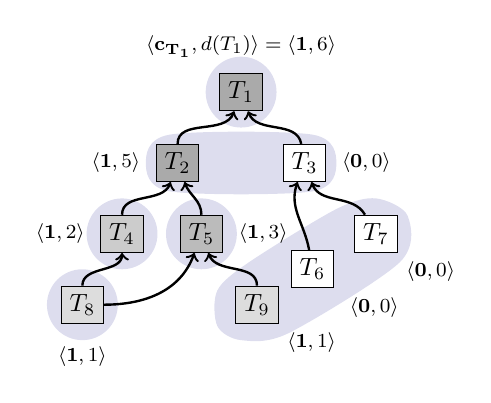
\begin{tikzpicture}[x=1.12cm, scale=0.9, every node/.append style={transform shape}]
    \begin{scope}[all/.style={draw, minimum height=0.5cm, minimum width=0.5cm},line width=0.08ex]
        \node[fill=lightgp, circle,minimum width=1cm] (pt1) at (0, 0) {};
        \node[fill=lightgp, circle,minimum width=1cm] (pt4) at (-1.5, -2) {};
        \node[fill=lightgp, circle,minimum width=1cm] (pt5) at (-0.5, -2) {};
        \node[fill=lightgp, circle,minimum width=1cm] (pt6) at (-2, -3) {};
        \fill[color=lightgp] plot[smooth cycle] coordinates { (1.2, -1) (0.9, -1.4) (-0.9, -1.4) (-1.2, -1) (-0.9, -0.6) (0.9, -0.6)} node (pt2) {};
        \fill[color=lightgp] plot[smooth cycle] coordinates {(2.1, -1.75) (2, -2.4) (0.6, -3.4) (0, -3.5) (-0.3, -3.3)(-0.3, -2.8) (0.1, -2.4) (1.2, -1.65) (1.7, -1.5) } node (pt3) {};
        \node[all, draw,fill=darkgray] (b0) at (0, 0) {$T_1$};
        \node[all, draw,fill=darkgray] (b1) at (-0.8, -1) {$T_2$};
        \node[all, draw,fill=white] (b2) at (0.8, -1) {$T_3$};
        \node[all, draw,fill=medgray] (b3) at (-1.5, -2) {$T_4$};
        \node[all, draw,fill=medgray2] (b4) at (-0.5, -2) {$T_5$};
        \node[all, draw,fill=white] (b5) at (0.9, -2.5) {$T_6$};
        \node[all, draw,fill=white] (b6) at (1.7, -2) {$T_7$};
        \node[all, draw,fill=lightgray] (b7) at (-2, -3) {$T_8$};
        \node[all, draw,fill=lightgray] (b8) at (0.2, -3) {$T_9$};
        \begin{scope}[line width=0.2ex]
        \path[->] (b1) edge[out=90, in=-110] node[sloped,above] {} (b0) ;
        \path[->] (b2) edge[out=100, in=-70] node[sloped,above] {} (b0) ;
        \path[->] (b3) edge[out=90, in=-110] node[sloped,above] {} (b1) ;
        \path[->] (b4) edge[out=90, in=-70] node[sloped,above] {} (b1) ;
        \path[->] (b5) edge[out=100, in=-110] node[sloped,above] {} (b2) ;
        \path[->] (b6) edge[out=120, in=-70] node[sloped,above] {} (b2) ;
        \path[->] (b7) edge[out=90, in=-90] node[sloped,above] {} (b3) ;
        \path[->] (b7) edge[out=0, in=-110] node[sloped,above] {} (b4) ;
        \path[->] (b8) edge[out=90, in=-70] node[sloped,above] {} (b4) ;
        \end{scope}
        %\node[] (p1) at (3, 0.5) {\footnotesize$\mathcal{P}_{T_1}$} ;
        %\node[] (p2) at (3, 0) {\footnotesize$\mathcal{P}_{T_2} = \mathcal{P}_{T_3}$};
        %\node[] (p3) at (3, -0.5) {\footnotesize$\mathcal{P}_{T_9} = \mathcal{P}_{T_6} = \mathcal{P}_{T_7}$};
        %\begin{scope}[color=darkgray,dashed,line width=0.2ex]
        %\path[->] (p1) edge[out=180, in=0] node[sloped,above] {} (pt1) ;
        %\path[->] (p2) edge[out=180, in=60] node[sloped,above] {} (pt2) ;
        %\path[->] (p3) edge[out=-90, in=30] node[sloped,above] {} (pt3) ;
        %\end{scope}

        \node[anchor=south, yshift=0.1cm] at (b0.north) {\footnotesize$\langle \mathbf{c_{T_1}}, d(T_1) \rangle = \langle\mathbf{1}, 6\rangle$};
        \node[anchor=east,xshift=-0.1cm] at (b1.west) {\footnotesize$\langle \mathbf{1}, 5 \rangle$};
        \node[anchor=west,xshift=0.1cm] at (b2.east) {\footnotesize$\langle \mathbf{0}, 0 \rangle$};
        \node[anchor=east,xshift=-0.1cm] at (b3.west) {\footnotesize$\langle \mathbf{1}, 2 \rangle$};
        \node[anchor=west,xshift=0.1cm] at (b4.east) {\footnotesize$\langle \mathbf{1}, 3 \rangle$};
        \node[anchor=north west,xshift=0.1cm] at (b5.south east) {\footnotesize$\langle \mathbf{0}, 0 \rangle$};
        \node[anchor=north west] at (b6.south east) {\footnotesize$\langle \mathbf{0}, 0 \rangle$};
        \node[anchor=north west] at (b8.south east) {\footnotesize$\langle \mathbf{1}, 1 \rangle$};
        \node[anchor=north,yshift=-0.2cm] at (b7.south) {\footnotesize$\langle \mathbf{1}, 1 \rangle$};
        
    \end{scope}
\end{tikzpicture}

    \captionof{figure}{Example of chits and confidence values.  Darker boxes mean transactions with greater confidence values.}\label{fig:dag-cd}
\end{center}

In Figure~\ref{fig:dag-cd}, notation $\langle c_T, d(T)\rangle$ is the pair of voting result
$c_T$ and confidence $d(T)$ tagged to each transaction $T$.  Notice $c_T$ is
immutable after voting, while $d(T)$ is subject to change as the DAG grows.
Given the
voting rule, the system will topple over to a single transaction in each
conflict set.  For example, in set~2, $T_2$ has much larger confidence than
$T_3$ so it will likely be voted $c_{T_2} = 1$ in the future.

%YYY
%what I really want to write here is that there exists some equation X, that gives us the probability that
%T will get reverted. As a probabilistic protocol, we cannot provide a clear commit point. So applications
%can at best decide to commit a transaction when the probability of reversion is low enough for their use.
%In this sense, we are exactly like Nakamoto consensus.
%There should be a function $\gamma$ that gives us the probability of reversion.

Finally, unlike deterministic protocols, Snowball leaves the finalization of a
transaction to the application, by providing a predicate associated with
probabilistic guarantee.  The \textsc{isCommitted} predicate becomes true when $T$ is the
preferred transaction in its conflict set, and the confidence $d(T)$ exceeds
the sum of the confidence for all conflicting transactions by a constant
$\beta$ (XXX change here). As a probabilistic protocol, the truth of this predicate could be flipped, though,
with very low probability depending on the security parameter $\beta$. The
application using Snowball achieves the finality by choosing the appropriate
security parameters that deliver the desired probabilistic bound of safety:
given the observation of \textsc{isCommitted} being true, the
probability of all correct nodes eventually stick to true.

%The Snowball protocol relies on two security parameters $\alpha$ and $\beta$.
%XXX describe alpha and beta, and how they are selected based on desired probability of loss
%XXX if transactions carry monetary amounts, one can bound the actual dollar loss by multiplying
%XXX \gamma with the amount of the transaction.

The final outstanding component of the protocol is transaction generation, specifically, the choice of parents for a newly minted transactions.
We note that this choice does not affect the safety guarantees of the protocol, as discussed later in our analysis in Subsection \ref{subsec:safetyanalysis}. 
%Because for a particular transaction in the DAG, its confidence solely depends on the chits in its own progeny. 
%Moreover, since the \textsc{isCommitted} predicate is determined by the difference of confidence between transactions in the same conflict set, the only thing that matters in affecting the difference is which progeny set future transactions attach them to, rather than the microscopic DAG structure within the progeny sets.
However, parent selection can significantly affect the liveness of certain transactions, where transactions with badly chosen parents can remain stuck, forever unable to accrue the confidence required for commitment. 
In Section~\ref{sec:parent}, we provide three heuristics,
\emph{random}, \emph{frontier}, and \emph{adaptive}, and show that adaptive parent selection leads to good liveness properties that the \textsc{isCommitted} predicate will be probabilistically guaranteed to hold eventually for virtuous transactions.
%YYY what is good liveness?
A virtuous transaction is guaranteed to have a singleton conflict set consisting of just itself.

Figure~\ref{fig:gossipchain-ongen} shows the initialization of
a node's variables as well as what happens when a node learns of a
new transaction.  Section~\ref{sec:parent} discusses parent
selection from $\mathcal{T}$ for new transactions (which does not
affect safety).

\begin{figure}
\begin{center}
\begin{algorithmic}[1]
    \small
    \Procedure{init}{}
        \State $\mathcal{T} \coloneqq \emptyset$ \hspace{1ex}\textrm{// the set of known transactions}
        \State $\mathcal{Q} \coloneqq \emptyset$ \hspace{1ex}\textrm{// the set of polled transactions}
    \EndProcedure
    \Procedure{onGenerateTx}{$\mathrm{data}$}
        \State $\mathrm{edges} \coloneqq \{T' \gets T: T' \in \Call{parentSelection}{\mathcal{T}}\}$
        \State $T \coloneqq \texttt{Tx}(\mathrm{data}, \mathrm{edges})$
        \State $\mathcal{T} \coloneqq \mathcal{T} \cup \{T\}$
    \EndProcedure
    \Procedure{onReceiveTx}{$T$}
        \If{$T \notin \mathcal{T}$}
            \State $\mathcal{P}_T \coloneqq \mathcal{P}_T \cup \{T\}$
            \State $\mathcal{T} \coloneqq \mathcal{T} \cup \{T\}$
            \State $c_T \coloneqq 0$.
        \EndIf
    \EndProcedure
    \captionof{figure}{Transaction generation and bookkeeping.}\label{fig:gossipchain-ongen}
\end{algorithmic}
\end{center}
\end{figure}

% In Figure~\ref{fig:dag-conflicting-set}, there are 9 transactions and 6
% conflict sets. Solid edges represent parent relation and purple area stands for
% conflict set grouping.  Transaction $T_8$ has two parents $T_4$ and $T_5$ while
% the others only have one.

Figure~\ref{fig:gossipchain-main} shows the main loop of the core protocol.
In each iteration, the loop attempts to select a transaction $T$ that has not
yet been polled, but whose ancestors have all been polled.  (If no such
transaction exists, the loop will stall until a new transaction is
added to $\mathcal{T}$.)
The loop then selects $k$ peers and polls those peers.
If more than $\alpha k$ of those peers return a positive response,
the chit value is set to~1.  Then $T$ is added to the set $\mathcal{Q}$
so it will never be polled again by the node.
(The code that selects additional peers if some of the $k$ peers are
unresponsive is omitted for simplicity.)

\begin{figure}
\begin{center}
\small
\begin{algorithmic}[1]
    \Procedure{gossipChain}{}
        \While {\texttt{true}}
            \State \textrm{// select Tx with polled ancestors}
            \State\textrm{find  $T$ that satisfies }%\vspace*{-.6\baselineskip}
            $T \in \mathcal{T} \land T \notin \mathcal{Q}$
            %\begin{align*}\hspace{2ex}
            %    T \in \mathcal{T} &\land T \notin \mathcal{Q} \\
            %            &\land (\forall T', T' \gets T: T' \in \mathcal{Q})
            %\end{align*}
            \State \textrm{// randomly sample from the known nodes}
            \State $\mathcal{K} \coloneqq \texttt{sample}(\mathcal{N}, k)$
            \State $P \coloneqq \sum_{i \in \mathcal{K}}\texttt{poll}(i, T)$
            \If{$P > \alpha\cdot k$}
                \State $c_T \coloneqq 1$
            \EndIf
            \State\textrm{// otherwise, }$c_T$\textrm{ remains 0 forever}
            \State $\mathcal{Q} \coloneqq \mathcal{Q} \cup \{T\}$ \hspace {1ex} \textrm{// mark T as polled}
        \EndWhile
    \EndProcedure
    \captionof{figure}{The main gossip loop.}\label{fig:gossipchain-main}
\end{algorithmic}
\end{center}
\end{figure}

% TODO IMPORTANT The isPreferred must imply that T is polled, but current writing can be not polled. Also, do you do max over only polled transactions? 
\begin{figure}
\begin{center}
\small
\begin{algorithmic}[1]
    \Function{isPreferred}{$T$}
        \State \Return $d(T) = \max_{T' \in \mathcal{P}_T} d(T')$
    \EndFunction
    \Function{isStronglyPreferred}{$T$}
        \State \Return $\forall T'\in\mathcal{T}, T' \stackrel{*}{\gets} T: \Call{isPreferred}{T'}$
    \EndFunction
    \Procedure{onPoll}{$j, T$}
        \State \Call{onReceiveTx}{$T$}
        \If{\Call{isStronglyPreferred}{$T$}}
            \State $\Call{respond}{j, 1}$\hspace{2ex}\textrm{// vote yes}
        \Else
            \State $\Call{respond}{j, 0}$\hspace{2ex}\textrm{// vote no}
        \EndIf
    \EndProcedure
    \captionof{figure}{The voting rule.}\label{fig:gossipchain-onpoll}
\end{algorithmic}
\end{center}
\end{figure}

Figure~\ref{fig:gossipchain-onpoll} shows what happens when a node
receives a poll for a transaction $T$ from a peer $j$.
First it adds $T$ to $\mathcal{T}$, unless it already has it.
Then it determines if $T$ is currently strongly preferred.
If so, the node returns a positive response to peer $j$.
If not, the node returns a negative response.

\begin{figure}
\begin{center}
\begin{algorithmic}[1]
    \small
    \Function{isCommitted}{$T$}
        \State\Return
            \vspace*{-.8\baselineskip}
        \begin{align*}
            \Call{isPreferred}{T} &\land d(T) \\
            &- \sum_{T' \in \mathcal{P}_T, T' \neq T}{d(T')} \ge \beta
        \end{align*}
    \EndFunction
    \captionof{figure}{The commit condition.}\label{fig:gossipchain-diff-commit}
\end{algorithmic}
\end{center}
\end{figure}

Finally, Figure~\ref{fig:gossipchain-diff-commit} shows pseudo-code for
the commit decision for a transaction $T$.

\subsection{Parent Selection}
\label{sec:parent}

The goal of the parent selection policy is to yield a well-structured DAG that maximizes
the likelihood that virtuous transactions will be quickly accepted by the network. While this
policy will not affect the safety of the protocol, it plays a crucial role in determining
the shape and structure of the DAG, and affects liveness.

There are inherent trade-offs in the parent selection policy: selecting well-accepted parents make it
more likely for a transaction to find support, but can lead to vote dilution; as well, selecting more
recent parents at the frontier of the DAG can lead to stuck transactions, as the parents may turn out
to be in conflict and remain unsupported.  In the following discussion, we illustrate this dilemma.
We assume that every transaction will select a small number, $p$, of parents, provided as a protocol parameter.
We focus on the the selection of eligible parent set, from which a subset of size $p$ can be chosen at random.

Perhaps the simplest idea is to mint a fresh transactions with parents picked uniformly at random
among those transactions that are already well-accepted. Specifically, we can adopt the predicate
used in the voting rule to determine eligible parents on which a node would vote positively, as follows:
\[
    \mathcal{E} = \{T: \forall T\in\mathcal{T}, \textsc{isStronglyPreferred}(T)\}.
\]

But this strategy has the drawback that it can suffer from vote dilution and lead to starved transactions.
This heuristic will yield to large sets of eligible parents, consisting mostly of historical, old transactions.
When a node samples the transactions uniformly from $\mathcal{E}$, the resulting DAG
will have large, ever-increasing fan-out. Because new transactions will have scarce progenies,
the voting process will take a long time to build the required confidence on any given new transaction.

In contrast, efforts to reduce fan-out and control the shape of DAG by selecting the recent transactions at
decision frontier suffers from another problem. Most recent transactions will have very small (usually zero) $d$ values,
simply because they do not have enough descendants. Further, their conflict sets may not be well-distributed
and well-known across the network, leading to a parent attachment under a transaction that will never be supported.
This means the best transactions to choose lie somewhere near the frontier, but not too far deep in history.

In adaptive selection, a node starts at the frontier and retreats towards the genesis transaction until it finds an eligible parent.
The frontier transactions are those that currently do not have any children in the node's $\mathcal{T}$.
The set of strongly preferred transactions $\mathcal{E}$ is filtered by an additional criterion that the confidence should be larger than zero. This filters out transactions from unstable conflict set having zero confidence.
If there exist $p$ transactions in the filtered $\mathcal{E}$, then the adaptive selection will just yield them.
%YYY why isn't this bad, for the reasons in the previous paragraph?
Otherwise, the policy tries the parents of the transactions in $\mathcal{E}$, thus increasing the chance of finding more stabilized transactions as it retreats.
The retreating search will terminate when it reaches the genesis transaction.
Formally, the selected parents in this adaptive selection policy is precisely:

\begin{center}
\begin{algorithmic}[1]
    \small
    \Function{parentSelection}{$\mathcal{T}$}
        \State $\mathcal{E}' \coloneqq \{T: d(T) > 0, \forall T\in\mathcal{E}\}$.
        \State \Return $\{T: T \in \mathcal{E}' \land \forall T'\in\mathcal{T}, T \gets T', T' \notin \mathcal{E}'\}$.
    \EndFunction
    \captionof{figure}{Adaptive parent selection.}\label{fig:gossipchain-parent}
\end{algorithmic}
\end{center}
%YYY what are you memoizing and why does this help? Also, can't an attacker create a gazillion nodes at the frontier and dilute your efforts?
The formal definition involves checking the modified frontier condition each
time it retreats and reaches a vertex. In fact, each ``forall'' quantifier
demands an $O(|\mathcal{T}|)$ time, so the overall cost is
$O(|\mathcal{T}|^2)$. However, by doing search from the frontier with
memoization, the quadratic cost could be avoided. Moreover, using an
approximation technique in Section~\ref{sec:pruning}, it is possible to replace the
$|\mathcal{T}|$ by a constant number of transactions in practice.

Attackers cannot suddenly create a surge of vertices at the frontier to dilute
the progress of Snowball, because with the above policy, only the transactions
with positive confidence will be considered as parents. The polling happens via
gossiping, and each query has to wait for the response from $k$ randomly chosen
peers. The pace is then coordinated by all correct nodes. So even if an
attacker increases the fan-out of the DAG, those new vertices will not
get much attention unless its has confidence larger than zero, in which the
progress is not diluted.
